\newpage
\section{Logistic Regression}
\begin{flushleft}


Mittels Logistischer Regression lassen sich diskrete Phänomene klassifizieren. Die Funktion des Models ist wie folgt definiert:


$$ h_{\Theta}(x) = g(\Theta^{T}x) $$ 
$$ g(z) = \frac{1}{1 + e^{-z}} $$
$$ h_{\Theta}(x) = \frac{1}{1 + e^{-\Theta^{T}x}} $$

Die Funktion $g(x)$ ist hierbei die sogenannte Sigmoid (oder auch logistische) Funktion.

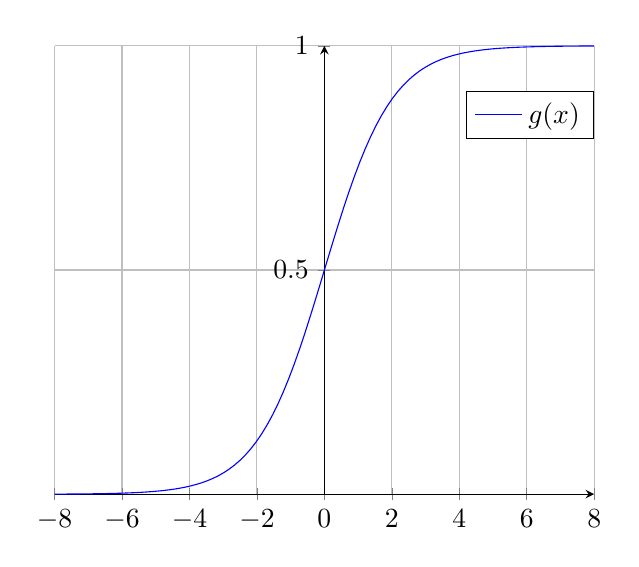
\begin{tikzpicture}[declare function={sigma(\x)=1/(1+exp(-\x));}]
\begin{axis}%
[
    grid=major,     
    xmin=-8,
    xmax=8,
    axis x line=bottom,
    ytick={0,.5,1},
    ymax=1,
    axis y line=middle,
    samples=100,
    domain=-8:8,
    legend style={at={(1,0.9)}}     
]
    \addplot[blue,mark=none]   (x,{sigma(x)});
    \legend{$g(x)$}
\end{axis}
\end{tikzpicture}

Der Wert $h_{\Theta}(x)$ wird als Wahrscheinlichkeit verstanden, dass der Output (y) positive ist für ein gegebener Eingabewert (x) parametrisiert mit $\Theta$.
\linebreak

Formal definiert:
$$h_{\Theta}(x) = P(y=1|x;\Theta)$$
Somit gilt:
$$ P(y=0|x;\Theta) = 1 - P(y=1|x;\Theta)$$


\end{flushleft}



